%% Based on a TeXnicCenter-Template by Gyorgy SZEIDL.
%%%%%%%%%%%%%%%%%%%%%%%%%%%%%%%%%%%%%%%%%%%%%%%%%%%%%%%%%%%%%

%------------------------------------------------------------
%
\documentclass{article}%
%Options -- Point size:  10pt (default), 11pt, 12pt
%        -- Paper size:  letterpaper (default), a4paper, a5paper, b5paper
%                        legalpaper, executivepaper
%        -- Orientation  (portrait is the default)
%                        landscape
%        -- Print size:  oneside (default), twoside
%        -- Quality      final(default), draft
%        -- Title page   notitlepage, titlepage(default)
%        -- Columns      onecolumn(default), twocolumn
%        -- Equation numbering (equation numbers on the right is the default)
%                        leqno
%        -- Displayed equations (centered is the default)
%                        fleqn (equations start at the same distance from the right side)
%        -- Open bibliography style (closed is the default)
%                        openbib
% For instance the command
%           \documentclass[a4paper,12pt,leqno]{article}
% ensures that the paper size is a4, the fonts are typeset at the size 12p
% and the equation numbers are on the left side
%
\usepackage{amsmath}%
\usepackage{amsfonts}%
\usepackage{amssymb}%
\usepackage{graphicx}
\usepackage{float}
\usepackage[utf8]{inputenc}
%-------------------------------------------
\newtheorem{theorem}{Theorem}
\newtheorem{acknowledgement}[theorem]{Acknowledgement}
\newtheorem{algorithm}[theorem]{Algorithm}
\newtheorem{axiom}[theorem]{Axiom}
\newtheorem{case}[theorem]{Case}
\newtheorem{claim}[theorem]{Claim}
\newtheorem{conclusion}[theorem]{Conclusion}
\newtheorem{condition}[theorem]{Condition}
\newtheorem{conjecture}[theorem]{Conjecture}
\newtheorem{corollary}[theorem]{Corollary}
\newtheorem{criterion}[theorem]{Criterion}
\newtheorem{definition}[theorem]{Definition}
\newtheorem{example}[theorem]{Example}
\newtheorem{exercise}[theorem]{Exercise}
\newtheorem{lemma}[theorem]{Lemma}
\newtheorem{notation}[theorem]{Notation}
\newtheorem{problem}[theorem]{Problem}
\newtheorem{proposition}[theorem]{Proposition}
\newtheorem{remark}[theorem]{Remark}
\newtheorem{solution}[theorem]{Solution}
\newtheorem{summary}[theorem]{Summary}
\newenvironment{proof}[1][Proof]{\textbf{#1.} }{\ \rule{0.5em}{0.5em}}

\begin{document}

\title{Proyecto Inteligencia Artificial II- Salida del Laberinto }
\author{Freen Esprint Jimenez Torres\thanks{Estudiante X semestre de ingenieria de sistemas}
\\Universidad de la Amazonia, Florencia}
\date{Noviembre 01, 2012}
\maketitle


\section{Descripción del problema}
Por definici\'on, un laberinto no es m\'as que una estructura formada por calles y encrucijadas, normalmente compleja, que intenta conseguir la confusi\'on en quien en ella se adentra. El nombre de laberinto proviene del lat\'in “labyrinthus” y del griego “lab\'yrinzos”. (Isabel Hern\'andez Fern\'andez, 2010)

Desde ese enfoque, la resoluci\'on de problemas se describe a menudo como una b\'usqueda en un enorme laberinto de posibilidades, un laberinto que describe el entorno. Para resolver exitosamente un problema se requiere explorar el laberinto de forma selectiva y con ello reducirlo a proporciones manejables. Pero los problemas que surgen a la hora de implementar una soluci\'on basada en b\'usqueda de laberintos son los siguientes entre otros:

\begin{itemize}
\item Las m\'aquinas a\'un no pueden reducir autom\'aticamente los problemas a proporciones manejables, es por ello que los seres humanos tienen que formular los problemas y proponer estrategias para encontrar su soluci\'on.
\item La complejidad que amerita encontrar la salida de un laberinto, donde su estructura es desconocida.
\end{itemize}

Debido a estos problemas, se debe hacer uso de t\'ecnicas de inteligencia artificial que proporcione las herramientas necesarias para la solucionar este tipo de inconvenientes.

\section{Estado del arte}
A continuaci\'on se plantean diferentes soluciones ya realizadas por algunos autores, en la resoluci\'on de laberintos por medio de la inteligencia artificial.
\subsection{T\'ECNICAS DE INTELIGENCIA ARTIFICIAL PARA LA SOLUCI\'ON DE LABERINTOS DE ESTRUCTURA DESCONOCIDA.}

En este trabajo se presentan las t\'ecnicas de b\'usqueda en amplitud y en profundidad, las cuales son t\'ecnicas de inteligencia artificial, para la soluci\'on de un problema de gran complejidad matem\'atica como lo es la soluci\'on de un laberinto de estructura desconocida.

El primer requisito que debe cumplir una buena estrategia de control es que cause alg\'un cambio, las estrategias de control que no causen cambio de estado nunca alcanzan la soluci\'on. El segundo requisito que debe cumplir una buena estrategia de control es que sea sistem\'atica.

Para tener una buena claridad de las estrategias de control en la soluci\'on de laberintos, se presenta en la Figura 1, a modo de ejemplo un laberinto que un m\'ovil, representado por un c\'irculo negro, desea solucionar; siendo la soluci\'on del laberinto el tri\'angulo negro. Las paredes del laberinto son cuadros grises y las posiciones en el laberinto se representan por una letra acompa\'nada por un n\'umero, de esta forma la posici\'on inicial se localiza en E9 y la posici\'on final en H1. En la figura 2 se presenta un \'arbol de b\'usqueda para el laberinto de la Figura 1. En la ra\'iz del \'arbol se encuentra el estado inicial, todas las ramificaciones de la ra\'iz se generan al aplicar cada una de las reglas al estado inicial. Cada bifurcaci\'on en una rama representa un punto del laberinto con varios caminos y una rama de la que no sale ninguna bifurcaci\'on puede ser un callej\'on sin salida o la soluci\'on. 


\begin{figure}[h]
  \begin{minipage}[b]{0.5\linewidth}
	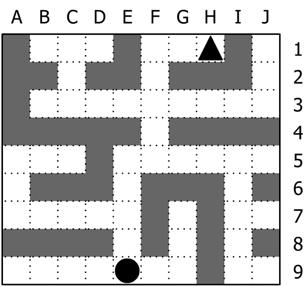
\includegraphics[width=0.65\textwidth]{laberinto.png}
     \caption{Laberinto}
  \end{minipage}%
  \begin{minipage}[b]{0.5\linewidth}
	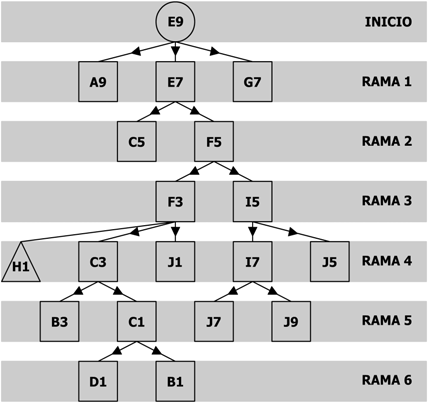
\includegraphics[width=0.75\textwidth]{busqueda.png}
     \caption{\'Arbol de b\'usqueda}
  \end{minipage}
\end{figure}

\subsection*{SOFTWARE DESARROLLADO}
Se desarroll\'o utilizando Wx Dev C++ un software para el estudio de los diferentes m\'etodos de soluci\'on de laberintos llamado Teseo. En la Figura 3 se presenta la interfaz gr\'afica de Teseo con la cual se pueden construir diferentes tipos de laberintos como el que se muestra a continuaci\'on:

\begin{figure}[h]
\centering
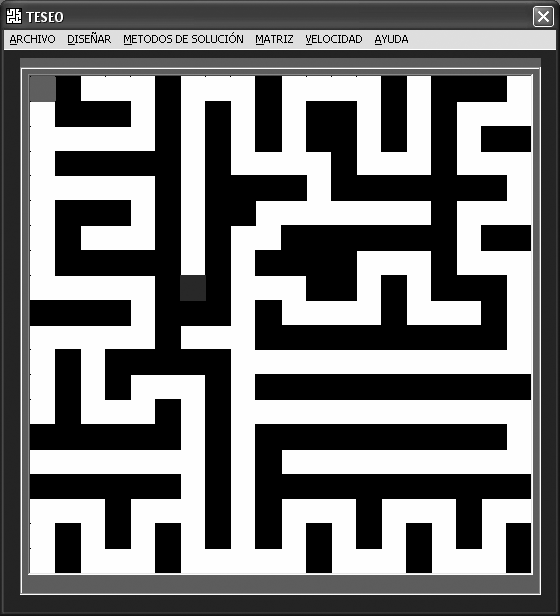
\includegraphics[width=0.45\textwidth]{dev.png}
     \caption{Laberinto}
\end{figure}

El m\'etodo de b\'usqueda en amplitud obtiene en promedio los mejores tiempos de soluci\'on a pesar de tener que recorrer todo el laberinto empleando m\'as memoria para realizar la b\'usqueda, por otro lado, la b\'usqueda en profundidad es m\'as aleatoria en cuanto al tiempo de soluci\'on, no obstante puede obtener mejores tiempos que la b\'usqueda en amplitud y menor cantidad de memoria, pero en promedio sus tiempos de b\'usqueda son mayores. Dependiendo del tipo de laberinto ingresado, cada m\'etodo empleado entrega una soluci\'on mejor que la otra.

\subsection {Buscador de caminos}
Aqu\'i tenemos un buscador de caminos, el ordenador podra encontrar una salida de el, buscara el mejor camino para salir y lo mostrara en pantalla, se puede modificar el punto de salida y el punto de llegada, osea el inicio del laberinto y el final, ademas en este buscador de caminos se puede modificar el laberinto, agregando o quitando muros, casillas.

El buscador de caminos consiste en un laberinto con una serie de obstaculos, se define un punto inicial y un punto final, y la inteligencia artificial buscara el camino mas optimo para llegar desde un punto a otro, la innovacion de este laberinto es que se puede modificar, cambiando por completo su estructura.

El buscador de caminos esta programado en flash, siendo la funcion de busqueda completamente action script.
\begin{figure}[H]
\centering
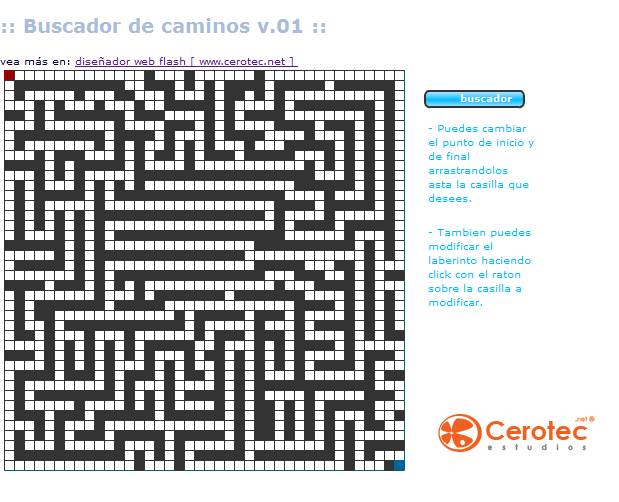
\includegraphics[width=1\textwidth]{buscador.png}
     \caption{Buscador de caminos}
\end{figure}

\section{Propuesta}
Como prop\'osito de la clase de Inteligencia Artificial II, se ha propuesto desarrollar un juego que implique el uso de t\'ecnicas computacionalmente inteligentes, dicho juego est\'a planteado de la siguiente forma:

\begin{enumerate}
\item El juego va constar de un laberinto y un personaje.
\item El laberinto va tener una entrada y una salida respectivamente.
\item Como m\'inimo, el laberinto debe tener un camino libre de obst\'aculos, que conecte la entrada con la salida.
\item El personaje tiene que estar en la capacidad de salir del laberinto autom\'aticamente.
\item El juego tiene la posibilidad de generar nuevos laberintos, donde la entrada y la salida se puedan mover a decisi\'on del usuario.
\item Por motivos de optimizaci\'on, el laberinto va a tener un ancho y alto predefinido de manera est\'atica.
\end{enumerate}

Para desarrollar este juego se piensa hacer uso de  t\'ecnicas computacionalmente inteligentes  como las “Redes neuronales supervisadas, altamente conexionistas”, ya que  las redes neuronales son las m\'as apropiadas, porque se basan en un aprendizaje continuo que a partir de unos par\'ametros de entrada y de salida, pueden ser entrenadas de manera adecuada, para as\'i satisfacer el requerimiento deseado. Adem\'as deben ser  altamente conexionistas para permitir un flujo de informaci\'on libre entre todas las neuronas, dando as\'i un mejor aprendizaje por parte de la red.

La red neuronal que se piensa a implementar es una red perceptron multicapa, ya que es una de las redes m\'as comunes a implementar y posee una gran capacidad de aprendizaje y adaptaci\'on en problemas computacionalmente complejos.

Adem\'as, La red neuronal va a tener tres capas implementadas, una capa de entrada, una capa oculta y una capa de salida, tal como lo muestra la siguiente figura:

\begin{figure}[h]
\centering
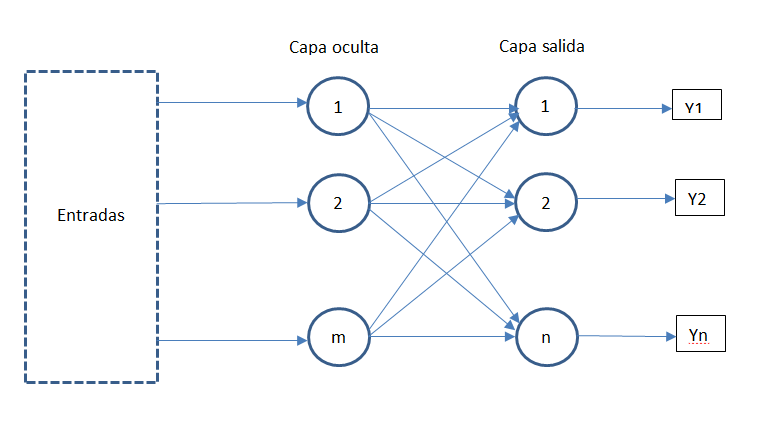
\includegraphics[width=1\textwidth]{redes.png}
     \caption{Arquitectura red neuronal}
\end{figure}

En la capa de entrada van a ir todos los posibles nodos por los cuales el personaje puede pasar.

En la capa oculta dependiendo el entrenamiento, el n\'umero de iteraciones y los resultados obtenidos, se ira a\'nadiendo o quitando neuronas, inicialmente se tiene la intenci\'on de arrancar con 5 neuronas en esta capa.

En la capa de salida se piensa hacer uso de m\'etodos de b\'usqueda por medio de inteligencia artificial, para encontrar la salida del laberinto m\'as \'optima. 

\end{document}
